\documentclass[12pt]{beamer}\usepackage[]{graphicx}\usepackage[]{color}
%% maxwidth is the original width if it is less than linewidth
%% otherwise use linewidth (to make sure the graphics do not exceed the margin)
\makeatletter
\def\maxwidth{ %
  \ifdim\Gin@nat@width>\linewidth
    \linewidth
  \else
    \Gin@nat@width
  \fi
}
\makeatother

\definecolor{fgcolor}{rgb}{0.345, 0.345, 0.345}
\newcommand{\hlnum}[1]{\textcolor[rgb]{0.686,0.059,0.569}{#1}}%
\newcommand{\hlstr}[1]{\textcolor[rgb]{0.192,0.494,0.8}{#1}}%
\newcommand{\hlcom}[1]{\textcolor[rgb]{0.678,0.584,0.686}{\textit{#1}}}%
\newcommand{\hlopt}[1]{\textcolor[rgb]{0,0,0}{#1}}%
\newcommand{\hlstd}[1]{\textcolor[rgb]{0.345,0.345,0.345}{#1}}%
\newcommand{\hlkwa}[1]{\textcolor[rgb]{0.161,0.373,0.58}{\textbf{#1}}}%
\newcommand{\hlkwb}[1]{\textcolor[rgb]{0.69,0.353,0.396}{#1}}%
\newcommand{\hlkwc}[1]{\textcolor[rgb]{0.333,0.667,0.333}{#1}}%
\newcommand{\hlkwd}[1]{\textcolor[rgb]{0.737,0.353,0.396}{\textbf{#1}}}%
\let\hlipl\hlkwb

\usepackage{framed}
\makeatletter
\newenvironment{kframe}{%
 \def\at@end@of@kframe{}%
 \ifinner\ifhmode%
  \def\at@end@of@kframe{\end{minipage}}%
  \begin{minipage}{\columnwidth}%
 \fi\fi%
 \def\FrameCommand##1{\hskip\@totalleftmargin \hskip-\fboxsep
 \colorbox{shadecolor}{##1}\hskip-\fboxsep
     % There is no \\@totalrightmargin, so:
     \hskip-\linewidth \hskip-\@totalleftmargin \hskip\columnwidth}%
 \MakeFramed {\advance\hsize-\width
   \@totalleftmargin\z@ \linewidth\hsize
   \@setminipage}}%
 {\par\unskip\endMakeFramed%
 \at@end@of@kframe}
\makeatother

\definecolor{shadecolor}{rgb}{.97, .97, .97}
\definecolor{messagecolor}{rgb}{0, 0, 0}
\definecolor{warningcolor}{rgb}{1, 0, 1}
\definecolor{errorcolor}{rgb}{1, 0, 0}
\newenvironment{knitrout}{}{} % an empty environment to be redefined in TeX

\usepackage{alltt}
\usepackage{graphicx}
\usepackage{tikz}
\setbeameroption{hide notes}
\setbeamertemplate{note page}[plain]
\usepackage{listings}

% get rid of junk
\usetheme{default}
\usefonttheme[onlymath]{serif}
\beamertemplatenavigationsymbolsempty
\hypersetup{pdfpagemode=UseNone} % don't show bookmarks on initial view

% named colors
\definecolor{offwhite}{RGB}{255,250,240}
\definecolor{gray}{RGB}{155,155,155}

\ifx\notescolors\undefined % slides

  \definecolor{foreground}{RGB}{80,80,80}
  \definecolor{background}{RGB}{255,255,255}
  \definecolor{title}{RGB}{255,199,0}
  \definecolor{subtitle}{RGB}{89,132,212}
  \definecolor{hilit}{RGB}{248,117,79}
  \definecolor{vhilit}{RGB}{255,111,207}
  \definecolor{lolit}{RGB}{200,200,200}
  \definecolor{lit}{RGB}{255,199,0}
  \definecolor{mdlit}{RGB}{89,132,212}
  \definecolor{link}{RGB}{248,117,79}

\else % notes
  \definecolor{background}{RGB}{255,255,255}
  \definecolor{foreground}{RGB}{24,24,24}
  \definecolor{title}{RGB}{27,94,134}
  \definecolor{subtitle}{RGB}{22,175,124}
  \definecolor{hilit}{RGB}{122,0,128}
  \definecolor{vhilit}{RGB}{255,0,128}
  \definecolor{lolit}{RGB}{95,95,95}
\fi
\definecolor{nhilit}{RGB}{128,0,128}  % hilit color in notes
\definecolor{nvhilit}{RGB}{255,0,128} % vhilit for notes

\newcommand{\hilit}{\color{hilit}}
\newcommand{\vhilit}{\color{vhilit}}
\newcommand{\nhilit}{\color{nhilit}}
\newcommand{\nvhilit}{\color{nvhilit}}
\newcommand{\lit}{\color{lit}}
\newcommand{\mdlit}{\color{mdlit}}
\newcommand{\lolit}{\color{lolit}}

% use those colors
\setbeamercolor{titlelike}{fg=title}
\setbeamercolor{subtitle}{fg=subtitle}
\setbeamercolor{frametitle}{fg=gray}
\setbeamercolor{structure}{fg=subtitle}
\setbeamercolor{institute}{fg=lolit}
\setbeamercolor{normal text}{fg=foreground,bg=background}
%\setbeamercolor{item}{fg=foreground} % color of bullets
%\setbeamercolor{subitem}{fg=hilit}
%\setbeamercolor{itemize/enumerate subbody}{fg=lolit}
\setbeamertemplate{itemize subitem}{{\textendash}}
\setbeamerfont{itemize/enumerate subbody}{size=\footnotesize}
\setbeamerfont{itemize/enumerate subitem}{size=\footnotesize}

% center title of slides
\setbeamertemplate{blocks}[rounded]
\setbeamertemplate{frametitle}[default][center]
% margins
\setbeamersize{text margin left=25pt,text margin right=25pt}

% page number
\setbeamertemplate{footline}{%
    \raisebox{5pt}{\makebox[\paperwidth]{\hfill\makebox[20pt]{\lolit
          \scriptsize\insertframenumber}}}\hspace*{5pt}}

% add a bit of space at the top of the notes page
\addtobeamertemplate{note page}{\setlength{\parskip}{12pt}}

% default link color
\hypersetup{colorlinks, urlcolor={link}}

\ifx\notescolors\undefined % slides
  % set up listing environment
  \lstset{language=bash,
          basicstyle=\ttfamily\scriptsize,
          frame=single,
          commentstyle=,
          backgroundcolor=\color{darkgray},
          showspaces=false,
          showstringspaces=false
          }
\else % notes
  \lstset{language=bash,
          basicstyle=\ttfamily\scriptsize,
          frame=single,
          commentstyle=,
          backgroundcolor=\color{offwhite},
          showspaces=false,
          showstringspaces=false
          }
\fi

% a few macros
\newcommand{\code}[1]{\texttt{#1}}
\newcommand{\hicode}[1]{{\hilit \texttt{#1}}}
\newcommand{\bb}[1]{\begin{block}{#1}}
\newcommand{\eb}{\end{block}}
\newcommand{\bi}{\begin{itemize}}
%\newcommand{\bbi}{\vspace{24pt} \begin{itemize} \itemsep8pt}
\newcommand{\bbi}{\vspace{4pt} \begin{itemize} \itemsep8pt}
\newcommand{\ei}{\end{itemize}}
\newcommand{\bv}{\begin{verbatim}}
\newcommand{\ev}{\end{verbatim}}
\newcommand{\ig}{\includegraphics}
\newcommand{\subt}[1]{{\footnotesize \color{subtitle} {#1}}}
\newcommand{\ttsm}{\tt \small}
\newcommand{\ttfn}{\tt \footnotesize}
\newcommand{\figh}[2]{\centerline{\includegraphics[height=#2\textheight]{#1}}}
\newcommand{\figw}[2]{\centerline{\includegraphics[width=#2\textwidth]{#1}}}



%------------------------------------------------
% end of header
%------------------------------------------------

\title{Basics of Functions}
\subtitle{STAT 133}
\author{\href{http://www.gastonsanchez.com}{Gaston Sanchez}}
\institute{\href{https://github.com/ucb-stat133/stat133-fall-2016}{\tt \scriptsize \color{foreground} github.com/ucb-stat133/stat133-fall-2016}}
\date{}
\IfFileExists{upquote.sty}{\usepackage{upquote}}{}
\begin{document}


{
  \setbeamertemplate{footline}{} % no page number here
  \frame{
    \titlepage
  } 
}

%------------------------------------------------

\begin{frame}
\frametitle{Functions}

R comes with many functions and packages that let us perform a wide variety of tasks. Sometimes, however, there's no function to do what we want to achieve. In these cases we need to create our own functions.

To talk about functions, we must first talk about \textbf{R expressions}

\end{frame}

%------------------------------------------------

\begin{frame}
\begin{center}
\Huge{\hilit{Expressions}}
\end{center}
\end{frame}

%------------------------------------------------

\begin{frame}[fragile]
\frametitle{Expressions}

\bb{R code is composed of a series of \textbf{expressions}}
\bbi
  \item assignment statements
  \item arithmetic expressions
  \item function calls
  \item conditional statements
  \item etc
\ei
\eb

\end{frame}

%------------------------------------------------

\begin{frame}[fragile]
\frametitle{Simple Expressions}
\begin{knitrout}\footnotesize
\definecolor{shadecolor}{rgb}{0.969, 0.969, 0.969}\color{fgcolor}\begin{kframe}
\begin{alltt}
\hlcom{# assignment statement}
\hlstd{a} \hlkwb{<-} \hlnum{12345}

\hlcom{# arithmetic expression}
\hlnum{525} \hlopt{+} \hlnum{34} \hlopt{-} \hlnum{280}

\hlcom{# function call}
\hlkwd{median}\hlstd{(}\hlnum{1}\hlopt{:}\hlnum{10}\hlstd{)}
\end{alltt}
\end{kframe}
\end{knitrout}
\end{frame}

%------------------------------------------------

\begin{frame}[fragile]
\frametitle{Expressions}

One way to separate expressions is with new lines:
\begin{knitrout}\footnotesize
\definecolor{shadecolor}{rgb}{0.969, 0.969, 0.969}\color{fgcolor}\begin{kframe}
\begin{alltt}
\hlstd{a} \hlkwb{<-} \hlnum{12345}
\hlnum{525} \hlopt{+} \hlnum{34} \hlopt{-} \hlnum{280}
\hlkwd{median}\hlstd{(}\hlnum{1}\hlopt{:}\hlnum{10}\hlstd{)}
\end{alltt}
\end{kframe}
\end{knitrout}

\end{frame}

%------------------------------------------------

\begin{frame}[fragile]
\frametitle{Grouping Expressions}

\bb{Constructs for grouping together expressions}
\bbi
  \item semicolons
  \item curly braces
\ei
\eb

\end{frame}

%------------------------------------------------

\begin{frame}[fragile]
\frametitle{Separating Expressions}

Simple expressions separated with new lines:
\begin{knitrout}\footnotesize
\definecolor{shadecolor}{rgb}{0.969, 0.969, 0.969}\color{fgcolor}\begin{kframe}
\begin{alltt}
\hlstd{a} \hlkwb{<-} \hlnum{10}
\hlstd{b} \hlkwb{<-} \hlnum{20}
\hlstd{d} \hlkwb{<-} \hlnum{30}
\end{alltt}
\end{kframe}
\end{knitrout}

\end{frame}

%------------------------------------------------

\begin{frame}[fragile]
\frametitle{Grouping Expressions}

Grouping expressions with semicolons:
\begin{knitrout}\footnotesize
\definecolor{shadecolor}{rgb}{0.969, 0.969, 0.969}\color{fgcolor}\begin{kframe}
\begin{alltt}
\hlstd{a} \hlkwb{<-} \hlnum{10}\hlstd{; b} \hlkwb{<-} \hlnum{20}\hlstd{; d} \hlkwb{<-} \hlnum{30}
\end{alltt}
\end{kframe}
\end{knitrout}

Although this is a perfectly valid expression, we recommend avoiding semicolons,
since they make code harder to review.

\end{frame}

%------------------------------------------------

\begin{frame}[fragile]
\frametitle{Grouping Expressions}

Grouping expressions with braces:
\begin{knitrout}\footnotesize
\definecolor{shadecolor}{rgb}{0.969, 0.969, 0.969}\color{fgcolor}\begin{kframe}
\begin{alltt}
\hlstd{\{}
  \hlstd{a} \hlkwb{<-} \hlnum{10}
  \hlstd{b} \hlkwb{<-} \hlnum{20}
  \hlstd{d} \hlkwb{<-} \hlnum{30}
\hlstd{\}}
\end{alltt}
\end{kframe}
\end{knitrout}

\end{frame}

%------------------------------------------------

\begin{frame}[fragile]
\frametitle{Grouping Expressions}

Multiple expressions in one line within braces:
\begin{knitrout}\footnotesize
\definecolor{shadecolor}{rgb}{0.969, 0.969, 0.969}\color{fgcolor}\begin{kframe}
\begin{alltt}
\hlstd{\{a} \hlkwb{<-} \hlnum{10}\hlstd{; b} \hlkwb{<-} \hlnum{20}\hlstd{; d} \hlkwb{<-} \hlnum{30}\hlstd{\}}
\end{alltt}
\end{kframe}
\end{knitrout}

Again, this piece of code is just for illustration purposes (don't write code
like this!)

\end{frame}

%------------------------------------------------

\begin{frame}[fragile]
\frametitle{Brackets and Braces in R}
\begin{center}
\ig[width=9cm]{images/braces.pdf}
\end{center}
\end{frame}

%------------------------------------------------

\begin{frame}[fragile]
\frametitle{Brackets and Braces}
\begin{knitrout}\footnotesize
\definecolor{shadecolor}{rgb}{0.969, 0.969, 0.969}\color{fgcolor}\begin{kframe}
\begin{alltt}
\hlcom{# brackets for objects}
\hlstd{dataset[}\hlnum{1}\hlopt{:}\hlnum{10}\hlstd{]}
\end{alltt}
\end{kframe}
\end{knitrout}

\pause
\begin{knitrout}\footnotesize
\definecolor{shadecolor}{rgb}{0.969, 0.969, 0.969}\color{fgcolor}\begin{kframe}
\begin{alltt}
\hlcom{# parentheses for functions}
\hlkwd{some_function}\hlstd{(dataset)}
\end{alltt}
\end{kframe}
\end{knitrout}

\pause
\begin{knitrout}\footnotesize
\definecolor{shadecolor}{rgb}{0.969, 0.969, 0.969}\color{fgcolor}\begin{kframe}
\begin{alltt}
\hlcom{# brackets for expressions}
\hlstd{\{}
  \hlnum{1} \hlopt{+} \hlnum{1}
  \hlkwd{mean}\hlstd{(}\hlnum{1}\hlopt{:}\hlnum{5}\hlstd{)}
  \hlstd{tbl} \hlkwb{<-} \hlkwd{read.csv}\hlstd{(}\hlstr{'datafile.csv'}\hlstd{)}
\hlstd{\}}
\end{alltt}
\end{kframe}
\end{knitrout}
\end{frame}

%------------------------------------------------

\begin{frame}[fragile]
\frametitle{Expressions}

\bbi
  \item A program is a set of instructions
  \item Programs are made up of expressions
  \item R expressions can be simple or compound
  \item \textbf{Every expression in R has a value}
\ei

\end{frame}

%------------------------------------------------

\begin{frame}[fragile]
\frametitle{Expressions}

\begin{knitrout}\footnotesize
\definecolor{shadecolor}{rgb}{0.969, 0.969, 0.969}\color{fgcolor}\begin{kframe}
\begin{alltt}
\hlcom{# Expressions can be simple statements:}
\hlnum{5} \hlopt{+} \hlnum{3}
\end{alltt}
\begin{verbatim}
## [1] 8
\end{verbatim}
\end{kframe}
\end{knitrout}

\begin{knitrout}\footnotesize
\definecolor{shadecolor}{rgb}{0.969, 0.969, 0.969}\color{fgcolor}\begin{kframe}
\begin{alltt}
\hlcom{# Expressions can also be compound:}
\hlstd{\{}\hlnum{5} \hlopt{+} \hlnum{3}\hlstd{;} \hlnum{4} \hlopt{*} \hlnum{2}\hlstd{;} \hlnum{1} \hlopt{+} \hlnum{1}\hlstd{\}}
\end{alltt}
\begin{verbatim}
## [1] 2
\end{verbatim}
\end{kframe}
\end{knitrout}

\end{frame}

%------------------------------------------------

\begin{frame}[fragile]
\frametitle{Expressions}

The value of an expression is the last evaluated statement:
\begin{knitrout}\footnotesize
\definecolor{shadecolor}{rgb}{0.969, 0.969, 0.969}\color{fgcolor}\begin{kframe}
\begin{alltt}
\hlcom{# value of an expression}
\hlstd{\{}\hlnum{5} \hlopt{+} \hlnum{3}\hlstd{;} \hlnum{4} \hlopt{*} \hlnum{2}\hlstd{;} \hlnum{1} \hlopt{+} \hlnum{1}\hlstd{\}}
\end{alltt}
\begin{verbatim}
## [1] 2
\end{verbatim}
\end{kframe}
\end{knitrout}
The result has the visibility of the last evaluation

\end{frame}

%------------------------------------------------

\begin{frame}[fragile]
\frametitle{Simple Expressions}

We use braces \{ \} to group the statements of an expression:
\begin{knitrout}\footnotesize
\definecolor{shadecolor}{rgb}{0.969, 0.969, 0.969}\color{fgcolor}\begin{kframe}
\begin{alltt}
\hlcom{# simple expression}
\hlstd{\{}\hlnum{5} \hlopt{+} \hlnum{3}\hlstd{\}}
\end{alltt}
\begin{verbatim}
## [1] 8
\end{verbatim}
\end{kframe}
\end{knitrout}
For simple expressions there is really no need to use braces.

\end{frame}

%------------------------------------------------

\begin{frame}[fragile]
\frametitle{Compound Expressions}

\bbi
  \item Compound expressions consist of multiple simple expressions
  \item Compound expressions require braces
  \item Simple expressions in a compound expression can be separated by semicolons or newlines
\ei

\end{frame}

%------------------------------------------------

\begin{frame}[fragile]
\frametitle{Compound Expressions}

Simple expressions in a compound expression separated by semicolons:
\begin{knitrout}\footnotesize
\definecolor{shadecolor}{rgb}{0.969, 0.969, 0.969}\color{fgcolor}\begin{kframe}
\begin{alltt}
\hlcom{# compound expression (just for demo purposes)}
\hlcom{# don't write code like this}
\hlstd{\{}\hlkwd{mean}\hlstd{(}\hlnum{1}\hlopt{:}\hlnum{10}\hlstd{);} \hlstr{'3'}\hlstd{;} \hlkwd{print}\hlstd{(}\hlstr{"hello"}\hlstd{);} \hlkwd{c}\hlstd{(}\hlnum{1}\hlstd{,} \hlnum{3}\hlstd{,} \hlnum{4}\hlstd{)\}}
\end{alltt}
\begin{verbatim}
## [1] "hello"
## [1] 1 3 4
\end{verbatim}
\end{kframe}
\end{knitrout}

\end{frame}

%------------------------------------------------

\begin{frame}[fragile]
\frametitle{Compound Expressions}

Simple expressions in a compound expression separated by newlines:
\begin{knitrout}\footnotesize
\definecolor{shadecolor}{rgb}{0.969, 0.969, 0.969}\color{fgcolor}\begin{kframe}
\begin{alltt}
\hlcom{# compound expression}
\hlstd{\{}
  \hlkwd{mean}\hlstd{(}\hlnum{1}\hlopt{:}\hlnum{10}\hlstd{)}
  \hlstr{'3'}
  \hlkwd{print}\hlstd{(}\hlstr{"hello"}\hlstd{)}
  \hlkwd{c}\hlstd{(}\hlnum{1}\hlstd{,} \hlnum{3}\hlstd{,} \hlnum{4}\hlstd{)}
\hlstd{\}}
\end{alltt}
\begin{verbatim}
## [1] "hello"
## [1] 1 3 4
\end{verbatim}
\end{kframe}
\end{knitrout}

You will use braces, but not like in this dummy example.

\end{frame}

%------------------------------------------------

\begin{frame}[fragile]
\frametitle{Compound Expressions}

It is possible to have assignments within compound expressions:
\begin{knitrout}\footnotesize
\definecolor{shadecolor}{rgb}{0.969, 0.969, 0.969}\color{fgcolor}\begin{kframe}
\begin{alltt}
\hlstd{\{}
  \hlstd{x} \hlkwb{<-} \hlnum{4}
  \hlstd{y} \hlkwb{<-} \hlstd{x}\hlopt{^}\hlnum{2}
  \hlstd{x} \hlopt{+} \hlstd{y}
\hlstd{\}}
\end{alltt}
\begin{verbatim}
## [1] 20
\end{verbatim}
\end{kframe}
\end{knitrout}

\end{frame}

%------------------------------------------------

\begin{frame}[fragile]
\frametitle{Compound Expressions}

The variables inside the braces can be used in later expressions
\begin{knitrout}\footnotesize
\definecolor{shadecolor}{rgb}{0.969, 0.969, 0.969}\color{fgcolor}\begin{kframe}
\begin{alltt}
\hlstd{z} \hlkwb{<-} \hlstd{\{x} \hlkwb{<-} \hlnum{4}\hlstd{; y} \hlkwb{<-} \hlstd{x}\hlopt{^}\hlnum{2}\hlstd{; x} \hlopt{+} \hlstd{y\}}
\hlstd{x}
\end{alltt}
\begin{verbatim}
## [1] 4
\end{verbatim}
\begin{alltt}
\hlstd{y}
\end{alltt}
\begin{verbatim}
## [1] 16
\end{verbatim}
\begin{alltt}
\hlstd{z}
\end{alltt}
\begin{verbatim}
## [1] 20
\end{verbatim}
\end{kframe}
\end{knitrout}

\end{frame}

%------------------------------------------------

\begin{frame}[fragile]
\frametitle{Compound Expressions}

\begin{knitrout}\footnotesize
\definecolor{shadecolor}{rgb}{0.969, 0.969, 0.969}\color{fgcolor}\begin{kframe}
\begin{alltt}
\hlcom{# simple expressions in newlines}
\hlstd{z} \hlkwb{<-} \hlstd{\{}
  \hlstd{x} \hlkwb{<-} \hlnum{4}
  \hlstd{y} \hlkwb{<-} \hlstd{x}\hlopt{^}\hlnum{2}
  \hlstd{x} \hlopt{+} \hlstd{y\}}
\hlstd{x}
\end{alltt}
\begin{verbatim}
## [1] 4
\end{verbatim}
\begin{alltt}
\hlstd{y}
\end{alltt}
\begin{verbatim}
## [1] 16
\end{verbatim}
\begin{alltt}
\hlstd{z}
\end{alltt}
\begin{verbatim}
## [1] 20
\end{verbatim}
\end{kframe}
\end{knitrout}

\end{frame}

%------------------------------------------------

\begin{frame}[fragile]
\frametitle{Using Expressions}

\bb{Expressions are typically used in}
\bbi
  \item Functions
  \item Flow control structures (e.g. \code{for} loop)
\ei
\eb

\end{frame}

%------------------------------------------------

\begin{frame}[fragile]
\frametitle{Compound Expressions}

Do not confuse a function call (having arguments in multiple lines) with a compound expression
\begin{knitrout}\footnotesize
\definecolor{shadecolor}{rgb}{0.969, 0.969, 0.969}\color{fgcolor}\begin{kframe}
\begin{alltt}
\hlcom{# this is NOT a compound expression}
\hlkwd{plot}\hlstd{(}\hlkwc{x} \hlstd{=} \hlkwd{runif}\hlstd{(}\hlnum{10}\hlstd{),} \hlkwc{y} \hlstd{=} \hlkwd{rnorm}\hlstd{(}\hlnum{10}\hlstd{),}
     \hlkwc{pch} \hlstd{=} \hlnum{19}\hlstd{,} \hlkwc{col} \hlstd{=} \hlstr{"#89F39A"}\hlstd{,} \hlkwc{cex} \hlstd{=} \hlnum{2}\hlstd{,}
     \hlkwc{main} \hlstd{=} \hlstr{"some plot"}\hlstd{,}
     \hlkwc{xlab} \hlstd{=} \hlstr{'x'}\hlstd{,} \hlkwc{ylab} \hlstd{=} \hlstr{'y'}\hlstd{)}
\end{alltt}
\end{kframe}
\end{knitrout}

\end{frame}

%------------------------------------------------

\begin{frame}
\begin{center}
\Huge{\hilit{Anatomy of a Function}}
\end{center}
\end{frame}

%------------------------------------------------

\begin{frame}[fragile]
\frametitle{Anatomy of a function}

{\hilit \code{function()}} allows us to create a function. It has the following structure:

\begin{knitrout}\footnotesize
\definecolor{shadecolor}{rgb}{0.969, 0.969, 0.969}\color{fgcolor}\begin{kframe}
\begin{alltt}
\hlstd{function_name} \hlkwb{<-} \hlkwa{function}\hlstd{(}\hlkwc{arg1}\hlstd{,} \hlkwc{arg2}\hlstd{,} \hlkwc{etc}\hlstd{)}
\hlstd{\{}
  \hlstd{expression_1}
  \hlstd{expression_2}
  \hlstd{...}
  \hlstd{expression_n}
\hlstd{\}}
\end{alltt}
\end{kframe}
\end{knitrout}

\end{frame}

%------------------------------------------------

\begin{frame}
\frametitle{Anatomy of a function}

\bi
  \item Generally we will give a name to a function
  \item A function takes one or more inputs (or none), known as as \textit{arguments}
  \item The expressions forming the operations comprise the body of the function
  \item Simple expression doesn't require braces
  \item Compound expressions are surround by braces
  \item Functions return a single \textit{value}
\ei

\end{frame}

%------------------------------------------------

\begin{frame}[fragile]
\frametitle{Function example}

A function that squares its argument:
\begin{knitrout}\footnotesize
\definecolor{shadecolor}{rgb}{0.969, 0.969, 0.969}\color{fgcolor}\begin{kframe}
\begin{alltt}
\hlstd{square} \hlkwb{<-} \hlkwa{function}\hlstd{(}\hlkwc{x}\hlstd{) \{}
  \hlstd{x}\hlopt{^}\hlnum{2}
\hlstd{\}}
\end{alltt}
\end{kframe}
\end{knitrout}

\pause
\bi
  \item the function's name is {\hilit \code{"square"}}
  \item it has one argument {\hilit \code{x}}
  \item the function's body consists of one simple expression
  \item it returns the value {\hilit \code{x * x}}  
\ei

\end{frame}

%------------------------------------------------

\begin{frame}[fragile]
\frametitle{Function example}

It works like any other function in R:
\begin{knitrout}\footnotesize
\definecolor{shadecolor}{rgb}{0.969, 0.969, 0.969}\color{fgcolor}\begin{kframe}
\begin{alltt}
\hlkwd{square}\hlstd{(}\hlnum{10}\hlstd{)}
\end{alltt}
\begin{verbatim}
## [1] 100
\end{verbatim}
\end{kframe}
\end{knitrout}

In this case, \code{square()} is also vectorized
\begin{knitrout}\footnotesize
\definecolor{shadecolor}{rgb}{0.969, 0.969, 0.969}\color{fgcolor}\begin{kframe}
\begin{alltt}
\hlkwd{square}\hlstd{(}\hlnum{1}\hlopt{:}\hlnum{5}\hlstd{)}
\end{alltt}
\begin{verbatim}
## [1]  1  4  9 16 25
\end{verbatim}
\end{kframe}
\end{knitrout}
Why is \code{square()} vectorized?

\end{frame}

%------------------------------------------------

\begin{frame}[fragile]
\frametitle{Function example}

Functions with a body consisting of a simple expression can be written with no braces (in one single line!):
\begin{knitrout}\footnotesize
\definecolor{shadecolor}{rgb}{0.969, 0.969, 0.969}\color{fgcolor}\begin{kframe}
\begin{alltt}
\hlstd{square} \hlkwb{<-} \hlkwa{function}\hlstd{(}\hlkwc{x}\hlstd{) x} \hlopt{*} \hlstd{x}

\hlkwd{square}\hlstd{(}\hlnum{10}\hlstd{)}
\end{alltt}
\begin{verbatim}
## [1] 100
\end{verbatim}
\end{kframe}
\end{knitrout}

\end{frame}

%------------------------------------------------

\begin{frame}[fragile]
\frametitle{}

If the body of a function is a compund expression we use braces:
\begin{knitrout}\footnotesize
\definecolor{shadecolor}{rgb}{0.969, 0.969, 0.969}\color{fgcolor}\begin{kframe}
\begin{alltt}
\hlstd{sum_sqr} \hlkwb{<-} \hlkwa{function}\hlstd{(}\hlkwc{x}\hlstd{,} \hlkwc{y}\hlstd{) \{}
  \hlstd{xy_sum} \hlkwb{<-} \hlstd{x} \hlopt{+} \hlstd{y}
  \hlstd{xy_ssqr} \hlkwb{<-} \hlstd{(xy_sum)}\hlopt{^}\hlnum{2}
  \hlkwd{list}\hlstd{(}\hlkwc{sum} \hlstd{= xy_sum,}
       \hlkwc{sumsqr} \hlstd{= xy_ssqr)}
\hlstd{\}}

\hlkwd{sum_sqr}\hlstd{(}\hlnum{3}\hlstd{,} \hlnum{5}\hlstd{)}
\end{alltt}
\begin{verbatim}
## $sum
## [1] 8
## 
## $sumsqr
## [1] 64
\end{verbatim}
\end{kframe}
\end{knitrout}

\end{frame}

%------------------------------------------------

\begin{frame}[fragile]
\frametitle{Function example}

Once defined, functions can be used in other function definitions:
\begin{knitrout}\footnotesize
\definecolor{shadecolor}{rgb}{0.969, 0.969, 0.969}\color{fgcolor}\begin{kframe}
\begin{alltt}
\hlstd{sum_of_squares} \hlkwb{<-} \hlkwa{function}\hlstd{(}\hlkwc{x}\hlstd{) \{}
  \hlkwd{sum}\hlstd{(}\hlkwd{square}\hlstd{(x))}
\hlstd{\}}

\hlkwd{sum_of_squares}\hlstd{(}\hlnum{1}\hlopt{:}\hlnum{5}\hlstd{)}
\end{alltt}
\begin{verbatim}
## [1] 55
\end{verbatim}
\end{kframe}
\end{knitrout}

\end{frame}

%------------------------------------------------

\begin{frame}[fragile]
\frametitle{Area of a Rectangle}

A function which, given the values $l$ (length) and $w$ (width) computes the value $l \times w$
\begin{knitrout}\footnotesize
\definecolor{shadecolor}{rgb}{0.969, 0.969, 0.969}\color{fgcolor}\begin{kframe}
\begin{alltt}
\hlstd{area_rect} \hlkwb{<-} \hlkwa{function}\hlstd{(}\hlkwc{l}\hlstd{,} \hlkwc{w}\hlstd{) \{}
  \hlstd{l} \hlopt{*} \hlstd{w}
\hlstd{\}}
\end{alltt}
\end{kframe}
\end{knitrout}
\bi
  \item The formal arguments of the function are \code{l} and \code{w}
  \item The body of the function consists of the simple expression \code{l * w}
  \item The function has been assigned the name \code{"area\_rect"}
\ei

\end{frame}

%------------------------------------------------

\begin{frame}[fragile]
\frametitle{Nested Functions}

We can also define a function inside another function:
\begin{knitrout}\footnotesize
\definecolor{shadecolor}{rgb}{0.969, 0.969, 0.969}\color{fgcolor}\begin{kframe}
\begin{alltt}
\hlstd{getmax} \hlkwb{<-} \hlkwa{function}\hlstd{(}\hlkwc{a}\hlstd{) \{}
  \hlstd{maxpos} \hlkwb{<-} \hlkwa{function}\hlstd{(}\hlkwc{u}\hlstd{) \{}
    \hlkwd{which.max}\hlstd{(u)}
  \hlstd{\}}
  \hlkwd{list}\hlstd{(}\hlkwc{position} \hlstd{=} \hlkwd{maxpos}\hlstd{(a),}
       \hlkwc{value} \hlstd{=} \hlkwd{max}\hlstd{(a))}
\hlstd{\}}

\hlkwd{getmax}\hlstd{(}\hlkwd{c}\hlstd{(}\hlnum{2}\hlstd{,} \hlopt{-}\hlnum{4}\hlstd{,} \hlnum{6}\hlstd{,} \hlnum{10}\hlstd{, pi))}
\end{alltt}
\begin{verbatim}
## $position
## [1] 4
## 
## $value
## [1] 10
\end{verbatim}
\end{kframe}
\end{knitrout}

\end{frame}

%------------------------------------------------

\begin{frame}[fragile]
\frametitle{Function names}

\bb{Different ways to name functions}
\bi
  \item \code{squareroot()}
  \item \code{SquareRoot()}
  \item \code{squareRoot()}
  \item \code{square.root()}
  \item \code{square\_root()}
\ei
\eb

\end{frame}

%------------------------------------------------

\begin{frame}[fragile]
\frametitle{Function names}

\bb{Invalid names}
\bi
  \item \code{5quareroot()}: cannot begin with a number
  \item \code{\_sqrt()}: cannot begin with an underscore
  \item \code{square-root()}: cannot use hyphenated names
\ei
\eb

\bigskip
In addition, avoid using an already existing name, e.g. \code{sqrt()}

\end{frame}

%------------------------------------------------

\begin{frame}
\begin{center}
\Huge{\hilit{Function Output}}
\end{center}
\end{frame}

%------------------------------------------------

\begin{frame}
\frametitle{Function output}

\bbi
  \item The body of a function is an expression
  \item Remember that every expression has a value
  \item Hence every function has a value
\ei

\end{frame}

%------------------------------------------------

\begin{frame}
\frametitle{Function output}

The value of a function can be established in two ways:
\bi
  \item As the last evaluated simple expression (in the body)
  \item An explicitly \textbf{returned} value via {\hilit \code{return()}}
\ei

\end{frame}

%------------------------------------------------

\begin{frame}[fragile]
\frametitle{The \code{return()} command}

Sometimes the \code{return()} command is included to explicitly indicate the output of a function:

\begin{knitrout}\footnotesize
\definecolor{shadecolor}{rgb}{0.969, 0.969, 0.969}\color{fgcolor}\begin{kframe}
\begin{alltt}
\hlstd{add} \hlkwb{<-} \hlkwa{function}\hlstd{(}\hlkwc{x}\hlstd{,} \hlkwc{y}\hlstd{) \{}
  \hlstd{z} \hlkwb{<-} \hlstd{x} \hlopt{+} \hlstd{y}
  \hlkwd{return}\hlstd{(z)}
\hlstd{\}}

\hlkwd{add}\hlstd{(}\hlnum{2}\hlstd{,} \hlnum{3}\hlstd{)}
\end{alltt}
\begin{verbatim}
## [1] 5
\end{verbatim}
\end{kframe}
\end{knitrout}

\end{frame}

%------------------------------------------------

\begin{frame}[fragile]
\frametitle{The \code{return()} command}

If no \code{return()} is present, then R returns the last evaluated expression:

\begin{columns}[t]
\begin{column}{0.45\textwidth}

\begin{knitrout}\footnotesize
\definecolor{shadecolor}{rgb}{0.969, 0.969, 0.969}\color{fgcolor}\begin{kframe}
\begin{alltt}
\hlcom{# output with return()}
\hlstd{add} \hlkwb{<-} \hlkwa{function}\hlstd{(}\hlkwc{x}\hlstd{,} \hlkwc{y}\hlstd{) \{}
  \hlstd{z} \hlkwb{<-} \hlstd{x} \hlopt{+} \hlstd{y}
  \hlkwd{return}\hlstd{(z)}
\hlstd{\}}

\hlkwd{add}\hlstd{(}\hlnum{2}\hlstd{,} \hlnum{3}\hlstd{)}
\end{alltt}
\begin{verbatim}
## [1] 5
\end{verbatim}
\end{kframe}
\end{knitrout}
\end{column}

\begin{column}{0.45\textwidth}
\begin{knitrout}\footnotesize
\definecolor{shadecolor}{rgb}{0.969, 0.969, 0.969}\color{fgcolor}\begin{kframe}
\begin{alltt}
\hlcom{# output without return()}
\hlstd{add} \hlkwb{<-} \hlkwa{function}\hlstd{(}\hlkwc{x}\hlstd{,} \hlkwc{y}\hlstd{) \{}
  \hlstd{x} \hlopt{+} \hlstd{y}
\hlstd{\}}

\hlkwd{add}\hlstd{(}\hlnum{2}\hlstd{,} \hlnum{3}\hlstd{)}
\end{alltt}
\begin{verbatim}
## [1] 5
\end{verbatim}
\end{kframe}
\end{knitrout}
\end{column}
\end{columns}

\end{frame}

%------------------------------------------------

\begin{frame}[fragile]
\frametitle{The \code{return()} command}

Depending on what's returned or what's the last evaluated expression, just calling a function might not print anything:

\begin{columns}[t]
\begin{column}{0.45\textwidth}
\begin{knitrout}\footnotesize
\definecolor{shadecolor}{rgb}{0.969, 0.969, 0.969}\color{fgcolor}\begin{kframe}
\begin{alltt}
\hlcom{# nothing is printed}
\hlstd{add} \hlkwb{<-} \hlkwa{function}\hlstd{(}\hlkwc{x}\hlstd{,} \hlkwc{y}\hlstd{) \{}
  \hlstd{z} \hlkwb{<-} \hlstd{x} \hlopt{+} \hlstd{y}
\hlstd{\}}

\hlkwd{add}\hlstd{(}\hlnum{2}\hlstd{,} \hlnum{3}\hlstd{)}
\end{alltt}
\end{kframe}
\end{knitrout}
\end{column}

\begin{column}{0.45\textwidth}
\begin{knitrout}\footnotesize
\definecolor{shadecolor}{rgb}{0.969, 0.969, 0.969}\color{fgcolor}\begin{kframe}
\begin{alltt}
\hlcom{# output printed}
\hlstd{add} \hlkwb{<-} \hlkwa{function}\hlstd{(}\hlkwc{x}\hlstd{,} \hlkwc{y}\hlstd{) \{}
  \hlstd{z} \hlkwb{<-} \hlstd{x} \hlopt{+} \hlstd{y}
  \hlkwd{return}\hlstd{(z)}
\hlstd{\}}

\hlkwd{add}\hlstd{(}\hlnum{2}\hlstd{,} \hlnum{3}\hlstd{)}
\end{alltt}
\begin{verbatim}
## [1] 5
\end{verbatim}
\end{kframe}
\end{knitrout}
\end{column}
\end{columns}

\end{frame}

%------------------------------------------------

\begin{frame}[fragile]
\frametitle{The \code{return()} command}

Here we call the function and assign it to an object. The last evaluated expression has the same value in both cases:

\begin{columns}[t]
\begin{column}{0.45\textwidth}
\begin{knitrout}\footnotesize
\definecolor{shadecolor}{rgb}{0.969, 0.969, 0.969}\color{fgcolor}\begin{kframe}
\begin{alltt}
\hlcom{# nothing is printed}
\hlstd{add} \hlkwb{<-} \hlkwa{function}\hlstd{(}\hlkwc{x}\hlstd{,} \hlkwc{y}\hlstd{) \{}
  \hlstd{z} \hlkwb{<-} \hlstd{x} \hlopt{+} \hlstd{y}
\hlstd{\}}

\hlstd{a1} \hlkwb{<-} \hlkwd{add}\hlstd{(}\hlnum{2}\hlstd{,} \hlnum{3}\hlstd{)}
\hlstd{a1}
\end{alltt}
\begin{verbatim}
## [1] 5
\end{verbatim}
\end{kframe}
\end{knitrout}
\end{column}

\begin{column}{0.45\textwidth}
\begin{knitrout}\footnotesize
\definecolor{shadecolor}{rgb}{0.969, 0.969, 0.969}\color{fgcolor}\begin{kframe}
\begin{alltt}
\hlcom{# output printed}
\hlstd{add} \hlkwb{<-} \hlkwa{function}\hlstd{(}\hlkwc{x}\hlstd{,} \hlkwc{y}\hlstd{) \{}
  \hlstd{z} \hlkwb{<-} \hlstd{x} \hlopt{+} \hlstd{y}
  \hlkwd{return}\hlstd{(z)}
\hlstd{\}}

\hlstd{a2} \hlkwb{<-} \hlkwd{add}\hlstd{(}\hlnum{2}\hlstd{,} \hlnum{3}\hlstd{)}
\hlstd{a2}
\end{alltt}
\begin{verbatim}
## [1] 5
\end{verbatim}
\end{kframe}
\end{knitrout}
\end{column}
\end{columns}

\end{frame}

%------------------------------------------------

\begin{frame}[fragile]
\frametitle{The \code{return()} command}

If no \code{return()} is present, then R returns the last evaluated expression:

\begin{columns}[t]
\begin{column}{0.45\textwidth}
\begin{knitrout}\footnotesize
\definecolor{shadecolor}{rgb}{0.969, 0.969, 0.969}\color{fgcolor}\begin{kframe}
\begin{alltt}
\hlstd{add1} \hlkwb{<-} \hlkwa{function}\hlstd{(}\hlkwc{x}\hlstd{,} \hlkwc{y}\hlstd{) \{}
  \hlstd{x} \hlopt{+} \hlstd{y}
\hlstd{\}}

\hlstd{add2} \hlkwb{<-} \hlkwa{function}\hlstd{(}\hlkwc{x}\hlstd{,} \hlkwc{y}\hlstd{) \{}
  \hlstd{z} \hlkwb{<-} \hlstd{x} \hlopt{+} \hlstd{y}
  \hlstd{z}
\hlstd{\}}
\end{alltt}
\end{kframe}
\end{knitrout}
\end{column}

\begin{column}{0.45\textwidth}
\begin{knitrout}\footnotesize
\definecolor{shadecolor}{rgb}{0.969, 0.969, 0.969}\color{fgcolor}\begin{kframe}
\begin{alltt}
\hlstd{add3} \hlkwb{<-} \hlkwa{function}\hlstd{(}\hlkwc{x}\hlstd{,} \hlkwc{y}\hlstd{) \{}
  \hlstd{z} \hlkwb{<-} \hlstd{x} \hlopt{+} \hlstd{y}
\hlstd{\}}

\hlstd{add4} \hlkwb{<-} \hlkwa{function}\hlstd{(}\hlkwc{x}\hlstd{,} \hlkwc{y}\hlstd{) \{}
  \hlstd{z} \hlkwb{<-} \hlstd{x} \hlopt{+} \hlstd{y}
  \hlkwd{return}\hlstd{(z)}
\hlstd{\}}
\end{alltt}
\end{kframe}
\end{knitrout}
\end{column}
\end{columns}

\end{frame}

%------------------------------------------------

\begin{frame}[fragile]
\frametitle{The \code{return()} command}

\code{return()} can be useful when the output may be obtained in the middle of the function's body

\begin{columns}[t]
\begin{column}{0.55\textwidth}
\begin{knitrout}\footnotesize
\definecolor{shadecolor}{rgb}{0.969, 0.969, 0.969}\color{fgcolor}\begin{kframe}
\begin{alltt}
\hlstd{f} \hlkwb{<-} \hlkwa{function}\hlstd{(}\hlkwc{x}\hlstd{,} \hlkwc{y}\hlstd{,} \hlkwc{add} \hlstd{=} \hlnum{TRUE}\hlstd{) \{}
  \hlkwa{if} \hlstd{(add) \{}
    \hlkwd{return}\hlstd{(x} \hlopt{+} \hlstd{y)}
  \hlstd{\}} \hlkwa{else} \hlstd{\{}
    \hlkwd{return}\hlstd{(x} \hlopt{-} \hlstd{y)}
  \hlstd{\}}
\hlstd{\}}
\end{alltt}
\end{kframe}
\end{knitrout}
\end{column}

\begin{column}{0.35\textwidth}
\begin{knitrout}\footnotesize
\definecolor{shadecolor}{rgb}{0.969, 0.969, 0.969}\color{fgcolor}\begin{kframe}
\begin{alltt}
\hlkwd{f}\hlstd{(}\hlnum{2}\hlstd{,} \hlnum{3}\hlstd{,} \hlkwc{add} \hlstd{=} \hlnum{TRUE}\hlstd{)}
\end{alltt}
\begin{verbatim}
## [1] 5
\end{verbatim}
\begin{alltt}
\hlkwd{f}\hlstd{(}\hlnum{2}\hlstd{,} \hlnum{3}\hlstd{,} \hlkwc{add} \hlstd{=} \hlnum{FALSE}\hlstd{)}
\end{alltt}
\begin{verbatim}
## [1] -1
\end{verbatim}
\end{kframe}
\end{knitrout}
\end{column}
\end{columns}

\end{frame}

%------------------------------------------------

\begin{frame}[fragile]
\frametitle{\code{return()} versus \code{print()}}

Often, R beginners use the function \code{print()} to indicate the output
of a function:

\begin{knitrout}\footnotesize
\definecolor{shadecolor}{rgb}{0.969, 0.969, 0.969}\color{fgcolor}\begin{kframe}
\begin{alltt}
\hlstd{add} \hlkwb{<-} \hlkwa{function}\hlstd{(}\hlkwc{x}\hlstd{,} \hlkwc{y}\hlstd{) \{}
  \hlstd{z} \hlkwb{<-} \hlstd{x} \hlopt{+} \hlstd{y}
  \hlkwd{print}\hlstd{(z)}
\hlstd{\}}

\hlkwd{add}\hlstd{(}\hlnum{2}\hlstd{,} \hlnum{3}\hlstd{)}
\end{alltt}
\begin{verbatim}
## [1] 5
\end{verbatim}
\end{kframe}
\end{knitrout}

\end{frame}

%------------------------------------------------

\begin{frame}[fragile]
\frametitle{\code{return()} versus \code{print()}}

\bbi
  \item The function \code{print()} is a \textbf{generic} method in R.
  \item This meeans that \code{print()} has a different behavior depending on
  its input
  \item Unless you want to print intermediate results while the function is
  being executed, there is no need to return the ouput via \code{print()}
\ei
\begin{knitrout}\footnotesize
\definecolor{shadecolor}{rgb}{0.969, 0.969, 0.969}\color{fgcolor}\begin{kframe}
\begin{alltt}
\hlstd{add} \hlkwb{<-} \hlkwa{function}\hlstd{(}\hlkwc{x}\hlstd{,} \hlkwc{y}\hlstd{) \{}
  \hlstd{z} \hlkwb{<-} \hlstd{x} \hlopt{+} \hlstd{y}
  \hlstd{z}  \hlcom{# no need to use print()}
\hlstd{\}}

\hlkwd{add}\hlstd{(}\hlnum{2}\hlstd{,} \hlnum{3}\hlstd{)}
\end{alltt}
\begin{verbatim}
## [1] 5
\end{verbatim}
\end{kframe}
\end{knitrout}

\end{frame}

%------------------------------------------------

\begin{frame}
\begin{center}
\Huge{\hilit{Function Arguments}}
\end{center}
\end{frame}

%------------------------------------------------

\begin{frame}[fragile]
\frametitle{Function arguments}

Functions can have any number of arguments (even zero arguments)
\begin{knitrout}\footnotesize
\definecolor{shadecolor}{rgb}{0.969, 0.969, 0.969}\color{fgcolor}\begin{kframe}
\begin{alltt}
\hlcom{# function with 2 arguments}
\hlstd{add} \hlkwb{<-} \hlkwa{function}\hlstd{(}\hlkwc{x}\hlstd{,} \hlkwc{y}\hlstd{) x} \hlopt{+} \hlstd{y}

\hlcom{# function with no arguments}
\hlstd{hi} \hlkwb{<-} \hlkwa{function}\hlstd{()} \hlkwd{print}\hlstd{(}\hlstr{"Hi there!"}\hlstd{)}

\hlkwd{hi}\hlstd{()}
\end{alltt}
\begin{verbatim}
## [1] "Hi there!"
\end{verbatim}
\end{kframe}
\end{knitrout}

\end{frame}

%------------------------------------------------

\begin{frame}[fragile]
\frametitle{Arguments}

Arguments can have default values
\begin{knitrout}\footnotesize
\definecolor{shadecolor}{rgb}{0.969, 0.969, 0.969}\color{fgcolor}\begin{kframe}
\begin{alltt}
\hlstd{hey} \hlkwb{<-} \hlkwa{function}\hlstd{(}\hlkwc{x} \hlstd{=} \hlstr{""}\hlstd{) \{}
  \hlkwd{cat}\hlstd{(}\hlstr{"Hey"}\hlstd{, x,} \hlstr{"\textbackslash{}nHow is it going?"}\hlstd{)}
\hlstd{\}}

\hlkwd{hey}\hlstd{()}
\end{alltt}
\begin{verbatim}
## Hey  
## How is it going?
\end{verbatim}
\begin{alltt}
\hlkwd{hey}\hlstd{(}\hlstr{"Gaston"}\hlstd{)}
\end{alltt}
\begin{verbatim}
## Hey Gaston 
## How is it going?
\end{verbatim}
\end{kframe}
\end{knitrout}

\end{frame}

%------------------------------------------------

\begin{frame}[fragile]
\frametitle{Arguments with no default values}

If you specify an argument with no default value, you must give it a value everytime you call the function, otherwise you'll get an error:
\begin{knitrout}\footnotesize
\definecolor{shadecolor}{rgb}{0.969, 0.969, 0.969}\color{fgcolor}\begin{kframe}
\begin{alltt}
\hlstd{sqr} \hlkwb{<-} \hlkwa{function}\hlstd{(}\hlkwc{x}\hlstd{) \{}
  \hlstd{x}\hlopt{^}\hlnum{2}
\hlstd{\}}

\hlkwd{sqr}\hlstd{()}
\end{alltt}


{\ttfamily\noindent\bfseries\color{errorcolor}{\#\# Error in sqr(): argument "{}x"{} is missing, with no default}}\end{kframe}
\end{knitrout}

\end{frame}

%------------------------------------------------

\begin{frame}[fragile]
\frametitle{Arguments with no default values}

Sometimes we don't want to give default values, but we also don't want to cause an error. We can use {\hilit \code{missing()}} to see if an argument is missing:

\begin{columns}[t]
\begin{column}{0.5\textwidth}
\begin{knitrout}\footnotesize
\definecolor{shadecolor}{rgb}{0.969, 0.969, 0.969}\color{fgcolor}\begin{kframe}
\begin{alltt}
\hlstd{abc} \hlkwb{<-} \hlkwa{function}\hlstd{(}\hlkwc{a}\hlstd{,} \hlkwc{b}\hlstd{,} \hlkwc{c} \hlstd{=} \hlnum{3}\hlstd{) \{}
  \hlkwa{if} \hlstd{(}\hlkwd{missing}\hlstd{(b)) \{}
    \hlstd{result} \hlkwb{<-} \hlstd{a} \hlopt{*} \hlnum{2} \hlopt{+} \hlstd{c}
  \hlstd{\}} \hlkwa{else} \hlstd{\{}
    \hlstd{result} \hlkwb{<-} \hlstd{a} \hlopt{*} \hlstd{b} \hlopt{+} \hlstd{c}
  \hlstd{\}}
  \hlstd{result}
\hlstd{\}}
\end{alltt}
\end{kframe}
\end{knitrout}
\end{column}

\begin{column}{0.4\textwidth}
\begin{knitrout}\footnotesize
\definecolor{shadecolor}{rgb}{0.969, 0.969, 0.969}\color{fgcolor}\begin{kframe}
\begin{alltt}
\hlkwd{abc}\hlstd{(}\hlnum{1}\hlstd{)}
\end{alltt}
\begin{verbatim}
## [1] 5
\end{verbatim}
\begin{alltt}
\hlkwd{abc}\hlstd{(}\hlnum{1}\hlstd{,} \hlnum{4}\hlstd{)}
\end{alltt}
\begin{verbatim}
## [1] 7
\end{verbatim}
\end{kframe}
\end{knitrout}
\end{column}
\end{columns}

\end{frame}

%------------------------------------------------

\begin{frame}[fragile]
\frametitle{Arguments with no default values}

You can also set an argument value to \code{NULL} if you don't want to specify a default value:
\begin{knitrout}\footnotesize
\definecolor{shadecolor}{rgb}{0.969, 0.969, 0.969}\color{fgcolor}\begin{kframe}
\begin{alltt}
\hlstd{abcd} \hlkwb{<-} \hlkwa{function}\hlstd{(}\hlkwc{a}\hlstd{,} \hlkwc{b} \hlstd{=} \hlnum{2}\hlstd{,} \hlkwc{c} \hlstd{=} \hlnum{3}\hlstd{,} \hlkwc{d} \hlstd{=} \hlkwa{NULL}\hlstd{) \{}
  \hlkwa{if} \hlstd{(}\hlkwd{is.null}\hlstd{(d)) \{}
    \hlstd{result} \hlkwb{<-} \hlstd{a} \hlopt{*} \hlstd{b} \hlopt{+} \hlstd{c}
  \hlstd{\}} \hlkwa{else} \hlstd{\{}
    \hlstd{result} \hlkwb{<-} \hlstd{a} \hlopt{*} \hlstd{b} \hlopt{+} \hlstd{c} \hlopt{*} \hlstd{d}
  \hlstd{\}}
  \hlstd{result}
\hlstd{\}}
\end{alltt}
\end{kframe}
\end{knitrout}

\end{frame}

%------------------------------------------------

\begin{frame}[fragile]
\frametitle{More arguments}

\begin{knitrout}\footnotesize
\definecolor{shadecolor}{rgb}{0.969, 0.969, 0.969}\color{fgcolor}\begin{kframe}
\begin{alltt}
\hlcom{# arguments with and without default values}
\hlstd{myplot} \hlkwb{<-} \hlkwa{function}\hlstd{(}\hlkwc{x}\hlstd{,} \hlkwc{y}\hlstd{,} \hlkwc{col} \hlstd{=} \hlstr{"#3488ff"}\hlstd{,} \hlkwc{pch} \hlstd{=} \hlnum{19}\hlstd{) \{}
  \hlkwd{plot}\hlstd{(x, y,} \hlkwc{col} \hlstd{= col,} \hlkwc{pch} \hlstd{= pch)}
\hlstd{\}}

\hlkwd{myplot}\hlstd{(}\hlnum{1}\hlopt{:}\hlnum{5}\hlstd{,} \hlnum{1}\hlopt{:}\hlnum{5}\hlstd{)}
\end{alltt}
\end{kframe}

{\centering 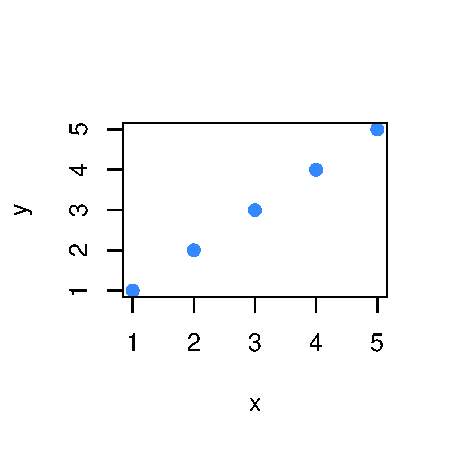
\includegraphics[width=.4\linewidth,height=.4\linewidth]{figure/unnamed-chunk-48-1} 

}



\end{knitrout}

\end{frame}

%------------------------------------------------

\begin{frame}[fragile]
\frametitle{More arguments}

\begin{knitrout}\footnotesize
\definecolor{shadecolor}{rgb}{0.969, 0.969, 0.969}\color{fgcolor}\begin{kframe}
\begin{alltt}
\hlcom{# arguments with and without default values}
\hlstd{myplot} \hlkwb{<-} \hlkwa{function}\hlstd{(}\hlkwc{x}\hlstd{,} \hlkwc{y}\hlstd{,} \hlkwc{col} \hlstd{=} \hlstr{"#3488ff"}\hlstd{,} \hlkwc{pch} \hlstd{=} \hlnum{19}\hlstd{) \{}
  \hlkwd{plot}\hlstd{(x, y,} \hlkwc{col} \hlstd{= col,} \hlkwc{pch} \hlstd{= pch)}
\hlstd{\}}
\end{alltt}
\end{kframe}
\end{knitrout}

\bi
  \item \code{x} and \code{y} have no default values
  \item \code{col} and \code{pch} have default values (but they can be changed)
\ei

\end{frame}

%------------------------------------------------

\begin{frame}[fragile]
\frametitle{More arguments}

\begin{knitrout}\footnotesize
\definecolor{shadecolor}{rgb}{0.969, 0.969, 0.969}\color{fgcolor}\begin{kframe}
\begin{alltt}
\hlcom{# changing default arguments}
\hlkwd{myplot}\hlstd{(}\hlnum{1}\hlopt{:}\hlnum{10}\hlstd{,} \hlnum{10}\hlopt{:}\hlnum{1}\hlstd{,} \hlkwc{col} \hlstd{=} \hlstr{"#994352"}\hlstd{,} \hlkwc{pch} \hlstd{=} \hlnum{18}\hlstd{)}
\end{alltt}
\end{kframe}

{\centering 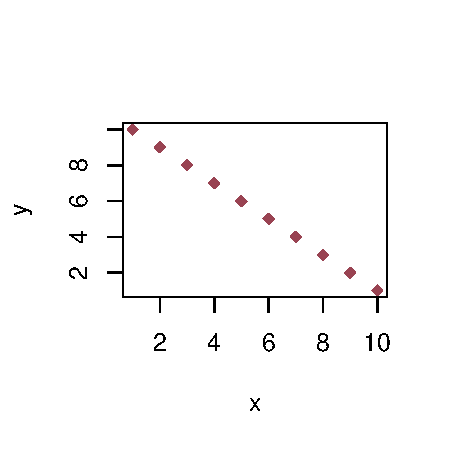
\includegraphics[width=.5\linewidth,height=.5\linewidth]{figure/unnamed-chunk-50-1} 

}



\end{knitrout}

\end{frame}

%------------------------------------------------

\begin{frame}
\begin{center}
\Huge{\hilit{Writing Functions}}
\end{center}
\end{frame}

%------------------------------------------------

\begin{frame}[fragile]
\frametitle{Writing Functions}

How to write functions?
\bi
  \item Always start simple with test toy-values
  \item Work first on what will be the body of the function
  \item Check out each step of the way
  \item Don't try to do much at once
  \item Create the function (i.e. encapsulate the body) once everything works
  \item Don't write long functions: write short / small functions (preferably less than 10 lines of code)
\ei

\end{frame}

%------------------------------------------------

\begin{frame}[fragile]
\frametitle{Variance Function Example}

The sample variance is given by the following formula:
$$
var(x) = \frac{1}{n-1} \sum_{i=1}^{n} (x_i - \bar{x})^2
$$

\end{frame}

%------------------------------------------------

\begin{frame}[fragile]
\frametitle{Variance Function Example}

\begin{knitrout}\footnotesize
\definecolor{shadecolor}{rgb}{0.969, 0.969, 0.969}\color{fgcolor}\begin{kframe}
\begin{alltt}
\hlcom{# start simple}
\hlstd{x} \hlkwb{<-} \hlnum{1}\hlopt{:}\hlnum{10}

\hlcom{# get working code}
\hlkwd{sum}\hlstd{((x} \hlopt{-} \hlkwd{mean}\hlstd{(x))}\hlopt{^}\hlnum{2}\hlstd{)} \hlopt{/} \hlstd{(}\hlkwd{length}\hlstd{(x)} \hlopt{-} \hlnum{1}\hlstd{)}
\end{alltt}
\begin{verbatim}
## [1] 9.166667
\end{verbatim}
\begin{alltt}
\hlcom{# test it: compare it to var()}
\hlkwd{var}\hlstd{(}\hlnum{1}\hlopt{:}\hlnum{10}\hlstd{)}
\end{alltt}
\begin{verbatim}
## [1] 9.166667
\end{verbatim}
\end{kframe}
\end{knitrout}

\end{frame}

%------------------------------------------------

\begin{frame}[fragile]
\frametitle{Variance Function Example}

\begin{knitrout}\footnotesize
\definecolor{shadecolor}{rgb}{0.969, 0.969, 0.969}\color{fgcolor}\begin{kframe}
\begin{alltt}
\hlcom{# encapsulate your code}
\hlstd{variance} \hlkwb{<-} \hlkwa{function}\hlstd{(}\hlkwc{x}\hlstd{) \{}
  \hlkwd{sum}\hlstd{((x} \hlopt{-} \hlkwd{mean}\hlstd{(x))}\hlopt{^}\hlnum{2}\hlstd{)} \hlopt{/} \hlstd{(}\hlkwd{length}\hlstd{(x)} \hlopt{-} \hlnum{1}\hlstd{)}
\hlstd{\}}

\hlcom{# check that it works}
\hlkwd{var}\hlstd{(}\hlnum{1}\hlopt{:}\hlnum{10}\hlstd{)}
\end{alltt}
\begin{verbatim}
## [1] 9.166667
\end{verbatim}
\end{kframe}
\end{knitrout}

\end{frame}

%------------------------------------------------

\begin{frame}[fragile]
\frametitle{Variance Function Example}

\begin{knitrout}\footnotesize
\definecolor{shadecolor}{rgb}{0.969, 0.969, 0.969}\color{fgcolor}\begin{kframe}
\begin{alltt}
\hlcom{# then consider less simple cases}
\hlkwd{variance} \hlstd{(}\hlkwd{runif}\hlstd{(}\hlnum{10}\hlstd{))}
\end{alltt}
\begin{verbatim}
## [1] 0.162643
\end{verbatim}
\begin{alltt}
\hlkwd{var}\hlstd{(}\hlkwd{rep}\hlstd{(}\hlnum{0}\hlstd{,} \hlnum{10}\hlstd{))}
\end{alltt}
\begin{verbatim}
## [1] 0
\end{verbatim}
\begin{alltt}
\hlkwd{var}\hlstd{(}\hlkwd{c}\hlstd{(}\hlnum{1}\hlopt{:}\hlnum{9}\hlstd{,} \hlnum{NA}\hlstd{))}
\end{alltt}
\begin{verbatim}
## [1] NA
\end{verbatim}
\end{kframe}
\end{knitrout}

\end{frame}

%------------------------------------------------

\begin{frame}[fragile]
\frametitle{Variance Function Example}

\begin{knitrout}\footnotesize
\definecolor{shadecolor}{rgb}{0.969, 0.969, 0.969}\color{fgcolor}\begin{kframe}
\begin{alltt}
\hlcom{# adapt it gradually}
\hlstd{variance} \hlkwb{<-} \hlkwa{function}\hlstd{(}\hlkwc{x}\hlstd{,} \hlkwc{na.rm} \hlstd{=} \hlnum{FALSE}\hlstd{) \{}
  \hlkwa{if} \hlstd{(na.rm) \{}
    \hlstd{x} \hlkwb{<-} \hlstd{x[}\hlopt{!}\hlkwd{is.na}\hlstd{(x)]}
  \hlstd{\}}
  \hlkwd{sum}\hlstd{((x} \hlopt{-} \hlkwd{mean}\hlstd{(x))}\hlopt{^}\hlnum{2}\hlstd{)} \hlopt{/} \hlstd{(}\hlkwd{length}\hlstd{(x)} \hlopt{-} \hlnum{1}\hlstd{)}
\hlstd{\}}

\hlkwd{variance}\hlstd{(}\hlkwd{c}\hlstd{(}\hlnum{1}\hlopt{:}\hlnum{9}\hlstd{,} \hlnum{NA}\hlstd{),} \hlkwc{na.rm} \hlstd{=} \hlnum{TRUE}\hlstd{)}
\end{alltt}
\begin{verbatim}
## [1] 7.5
\end{verbatim}
\end{kframe}
\end{knitrout}

Don't worry about \code{if()} conditionals, we'll talk about them later.

\end{frame}

%------------------------------------------------

\begin{frame}[fragile]
\frametitle{Writing Functions}

When writing functions:
\bi
  \item Choose meaningful names of functions
  \item Preferably a verb
  \item Choose meaningful names of arguments
  \item Think about the users (who will use the function)
  \item Think about extreme cases
  \item If a function is too long, maybe you need to split it
\ei

\end{frame}

%------------------------------------------------

\begin{frame}[fragile]
\frametitle{Names of functions}

Avoid this:
\begin{knitrout}\footnotesize
\definecolor{shadecolor}{rgb}{0.969, 0.969, 0.969}\color{fgcolor}\begin{kframe}
\begin{alltt}
\hlstd{f} \hlkwb{<-} \hlkwa{function}\hlstd{(}\hlkwc{x}\hlstd{,} \hlkwc{y}\hlstd{) \{}
  \hlstd{x} \hlopt{+} \hlstd{y}
\hlstd{\}}
\end{alltt}
\end{kframe}
\end{knitrout}

This is better
\begin{knitrout}\footnotesize
\definecolor{shadecolor}{rgb}{0.969, 0.969, 0.969}\color{fgcolor}\begin{kframe}
\begin{alltt}
\hlstd{add} \hlkwb{<-} \hlkwa{function}\hlstd{(}\hlkwc{x}\hlstd{,} \hlkwc{y}\hlstd{) \{}
  \hlstd{x} \hlopt{+} \hlstd{y}
\hlstd{\}}
\end{alltt}
\end{kframe}
\end{knitrout}

\end{frame}

%------------------------------------------------

\begin{frame}[fragile]
\frametitle{Names of arguments}

Give meaningful names to arguments:
\begin{knitrout}\footnotesize
\definecolor{shadecolor}{rgb}{0.969, 0.969, 0.969}\color{fgcolor}\begin{kframe}
\begin{alltt}
\hlcom{# Avoid this}
\hlstd{area_rect} \hlkwb{<-} \hlkwa{function}\hlstd{(}\hlkwc{x}\hlstd{,} \hlkwc{y}\hlstd{) \{}
  \hlstd{x} \hlopt{*} \hlstd{y}
\hlstd{\}}
\end{alltt}
\end{kframe}
\end{knitrout}

This is better
\begin{knitrout}\footnotesize
\definecolor{shadecolor}{rgb}{0.969, 0.969, 0.969}\color{fgcolor}\begin{kframe}
\begin{alltt}
\hlstd{area_rect} \hlkwb{<-} \hlkwa{function}\hlstd{(}\hlkwc{length}\hlstd{,} \hlkwc{width}\hlstd{) \{}
  \hlstd{length} \hlopt{*} \hlstd{width}
\hlstd{\}}
\end{alltt}
\end{kframe}
\end{knitrout}

\end{frame}

%------------------------------------------------

\begin{frame}[fragile]
\frametitle{Names of arguments}

Even better: give default values (whenever possible)
\begin{knitrout}\footnotesize
\definecolor{shadecolor}{rgb}{0.969, 0.969, 0.969}\color{fgcolor}\begin{kframe}
\begin{alltt}
\hlstd{area_rect} \hlkwb{<-} \hlkwa{function}\hlstd{(}\hlkwc{length} \hlstd{=} \hlnum{1}\hlstd{,} \hlkwc{width} \hlstd{=} \hlnum{1}\hlstd{) \{}
  \hlstd{length} \hlopt{*} \hlstd{width}
\hlstd{\}}

\hlcom{# default}
\hlkwd{area_rect}\hlstd{()}

\hlcom{# specifying argument values}
\hlkwd{area_rect}\hlstd{(}\hlkwc{length} \hlstd{=} \hlnum{10}\hlstd{,} \hlkwc{width} \hlstd{=} \hlnum{2}\hlstd{)}
\end{alltt}
\end{kframe}
\end{knitrout}

\end{frame}

%------------------------------------------------

\begin{frame}[fragile]
\frametitle{Meaningful Names to Arguments}

Avoid this:
\begin{knitrout}\footnotesize
\definecolor{shadecolor}{rgb}{0.969, 0.969, 0.969}\color{fgcolor}\begin{kframe}
\begin{alltt}
\hlcom{# what does this function do?}
\hlstd{ci} \hlkwb{<-} \hlkwa{function}\hlstd{(}\hlkwc{p}\hlstd{,} \hlkwc{r}\hlstd{,} \hlkwc{n}\hlstd{,} \hlkwc{ti}\hlstd{) \{}
  \hlstd{p} \hlopt{*} \hlstd{(}\hlnum{1} \hlopt{+} \hlstd{r}\hlopt{/}\hlstd{p)}\hlopt{^}\hlstd{(ti} \hlopt{*} \hlstd{p)}
\hlstd{\}}
\end{alltt}
\end{kframe}
\end{knitrout}

\pause
This is better:
\begin{knitrout}\footnotesize
\definecolor{shadecolor}{rgb}{0.969, 0.969, 0.969}\color{fgcolor}\begin{kframe}
\begin{alltt}
\hlcom{# OK}
\hlstd{compound_interest} \hlkwb{<-} \hlkwa{function}\hlstd{(}\hlkwc{principal}\hlstd{,} \hlkwc{rate}\hlstd{,} \hlkwc{periods}\hlstd{,} \hlkwc{time}\hlstd{) \{}
  \hlstd{principal} \hlopt{*} \hlstd{(}\hlnum{1} \hlopt{+} \hlstd{rate}\hlopt{/}\hlstd{periods)}\hlopt{^}\hlstd{(time} \hlopt{*} \hlstd{periods)}
\hlstd{\}}
\end{alltt}
\end{kframe}
\end{knitrout}

\end{frame}

%------------------------------------------------

\begin{frame}[fragile]
\frametitle{Meaningful Names to Arguments}

\begin{knitrout}\scriptsize
\definecolor{shadecolor}{rgb}{0.969, 0.969, 0.969}\color{fgcolor}\begin{kframe}
\begin{alltt}
\hlcom{# names of arguments}
\hlstd{compound_interest} \hlkwb{<-} \hlkwa{function}\hlstd{(}\hlkwc{principal} \hlstd{=} \hlnum{1}\hlstd{,} \hlkwc{rate} \hlstd{=} \hlnum{0.01}\hlstd{,}
                              \hlkwc{periods} \hlstd{=} \hlnum{1}\hlstd{,} \hlkwc{time} \hlstd{=} \hlnum{1}\hlstd{)}
\hlstd{\{}
  \hlstd{principal} \hlopt{*} \hlstd{(}\hlnum{1} \hlopt{+} \hlstd{rate}\hlopt{/}\hlstd{periods)}\hlopt{^}\hlstd{(time} \hlopt{*} \hlstd{periods)}
\hlstd{\}}

\hlkwd{compound_interest}\hlstd{(}\hlkwc{principal} \hlstd{=} \hlnum{100}\hlstd{,} \hlkwc{rate} \hlstd{=} \hlnum{0.05}\hlstd{,}
                  \hlkwc{periods} \hlstd{=} \hlnum{5}\hlstd{,} \hlkwc{time} \hlstd{=} \hlnum{1}\hlstd{)}

\hlkwd{compound_interest}\hlstd{(}\hlkwc{rate} \hlstd{=} \hlnum{0.05}\hlstd{,} \hlkwc{periods} \hlstd{=} \hlnum{5}\hlstd{,}
                  \hlkwc{time} \hlstd{=} \hlnum{1}\hlstd{,} \hlkwc{principal} \hlstd{=} \hlnum{100}\hlstd{)}

\hlkwd{compound_interest}\hlstd{(}\hlkwc{rate} \hlstd{=} \hlnum{0.05}\hlstd{,} \hlkwc{time} \hlstd{=} \hlnum{1}\hlstd{,}
                  \hlkwc{periods} \hlstd{=} \hlnum{5}\hlstd{,} \hlkwc{principal} \hlstd{=} \hlnum{100}\hlstd{)}
\end{alltt}
\end{kframe}
\end{knitrout}

\end{frame}


%------------------------------------------------

\begin{frame}[fragile]
\frametitle{Describing functions}

Also add a short description of what the arguments should be like. In this case, the description is outside the function
\begin{knitrout}\footnotesize
\definecolor{shadecolor}{rgb}{0.969, 0.969, 0.969}\color{fgcolor}\begin{kframe}
\begin{alltt}
\hlcom{# function for adding two numbers}
\hlcom{# x: number}
\hlcom{# y: number}
\hlstd{add} \hlkwb{<-} \hlkwa{function}\hlstd{(}\hlkwc{x}\hlstd{,} \hlkwc{y}\hlstd{) \{}
  \hlstd{x} \hlopt{+} \hlstd{y}
\hlstd{\}}
\end{alltt}
\end{kframe}
\end{knitrout}

\end{frame}

%------------------------------------------------

\begin{frame}[fragile]
\frametitle{Describing functions}

In this case, the description is inside the function
\begin{knitrout}\footnotesize
\definecolor{shadecolor}{rgb}{0.969, 0.969, 0.969}\color{fgcolor}\begin{kframe}
\begin{alltt}
\hlstd{add} \hlkwb{<-} \hlkwa{function}\hlstd{(}\hlkwc{x}\hlstd{,} \hlkwc{y}\hlstd{) \{}
  \hlcom{# function for adding two numbers}
  \hlcom{# x: number}
  \hlcom{# y: number}
  \hlstd{x} \hlopt{+} \hlstd{y}
\hlstd{\}}
\end{alltt}
\end{kframe}
\end{knitrout}

\end{frame}

%------------------------------------------------

\begin{frame}[fragile]
\frametitle{Describing functions}

\begin{knitrout}\footnotesize
\definecolor{shadecolor}{rgb}{0.969, 0.969, 0.969}\color{fgcolor}\begin{kframe}
\begin{alltt}
\hlcom{# description of arguments}
\hlstd{compound_interest} \hlkwb{<-} \hlkwa{function}\hlstd{(}\hlkwc{principal} \hlstd{=} \hlnum{1}\hlstd{,} \hlkwc{rate} \hlstd{=} \hlnum{0.01}\hlstd{,}
                              \hlkwc{periods} \hlstd{=} \hlnum{1}\hlstd{,} \hlkwc{time} \hlstd{=} \hlnum{1}\hlstd{)}
\hlstd{\{}
  \hlcom{# principal = Principal Amount}
  \hlcom{# rate = Annual Nominal Interest Rate as a decimal}
  \hlcom{# time = Time Involved in years}
  \hlcom{# periods = number of compounding periods per unit time}
  \hlstd{principal} \hlopt{*} \hlstd{(}\hlnum{1} \hlopt{+} \hlstd{rate}\hlopt{/}\hlstd{periods)}\hlopt{^}\hlstd{(time} \hlopt{*} \hlstd{periods)}
\hlstd{\}}
\end{alltt}
\end{kframe}
\end{knitrout}

\end{frame}

%------------------------------------------------

\end{document}
